%  !TeX  root  =  user_guide.tex  

%\section{Dxf2Shp Converter Plugin}
\section{Extension Convertisseur Dxf2Shp}

% when the revision of a section has been finalized, 
% comment out the following line:
%\updatedisclaimer

%The dxf2shape converter plugin can be used to convert vector data from DXF to Shapefile 
%format. It requires the following parameters to be specified before running:
L'extension Convertisseur dxf2shape permet de convertir des données 
vectorielles du format DXF au format shapefile (SHP). Avant d'être exécutée, 
elle requiert les réglages suivants:

%\begin{itemize}
%\item \textbf{Input DXF file}: Enter path to the DXF file to be converted
%\item \textbf{Output Shp file}: Enter desired name of the Shapefile to be created
%\item \textbf{Output file type}: Specify the geometry type of the output Shapefile. 
%Currently supported types are polyline, polygone, and point.
%\item \textbf{Export text labels}: When this checkbox is enabled, an additional Shapefile point layer will be created, and the associated dbf table will contain information about the "TEXT" fields found in the dxf file, and the text strings themselves.
%\end{itemize}
\begin{description}
\item[Fichier DXF :] Entrer la localisation du fichier DXF à convertir
\item[Fichier en sortie :] Entrer le nom souhaité du fichier shape à créer
%===> Dans l'interface, le nom du champ n'a pas été traduit en français
\item[Type de fichier de sortie :] Specifier le type géométrique du 
shapefile créé. 
Les formats implémentés pour le moment sont polyligne, polygone et point.
\item[Exporter les étiquettes :] Si cette case est cochée, une couche 
supplémentaire shapefile de type point sera créée et la table dbf associée 
contiendra des informations à propos des champs "TEXT" trouvés dans le fichier 
dxf ainsi que les chaînes de caractères elles-mêmes.
\end{description}

%\begin{figure}[ht]
%   \begin{center}
%   \caption{Dxf2Shape Converter Plugin \nixcaption}\label{fig:dxf2shape_dialog}\smallskip
%   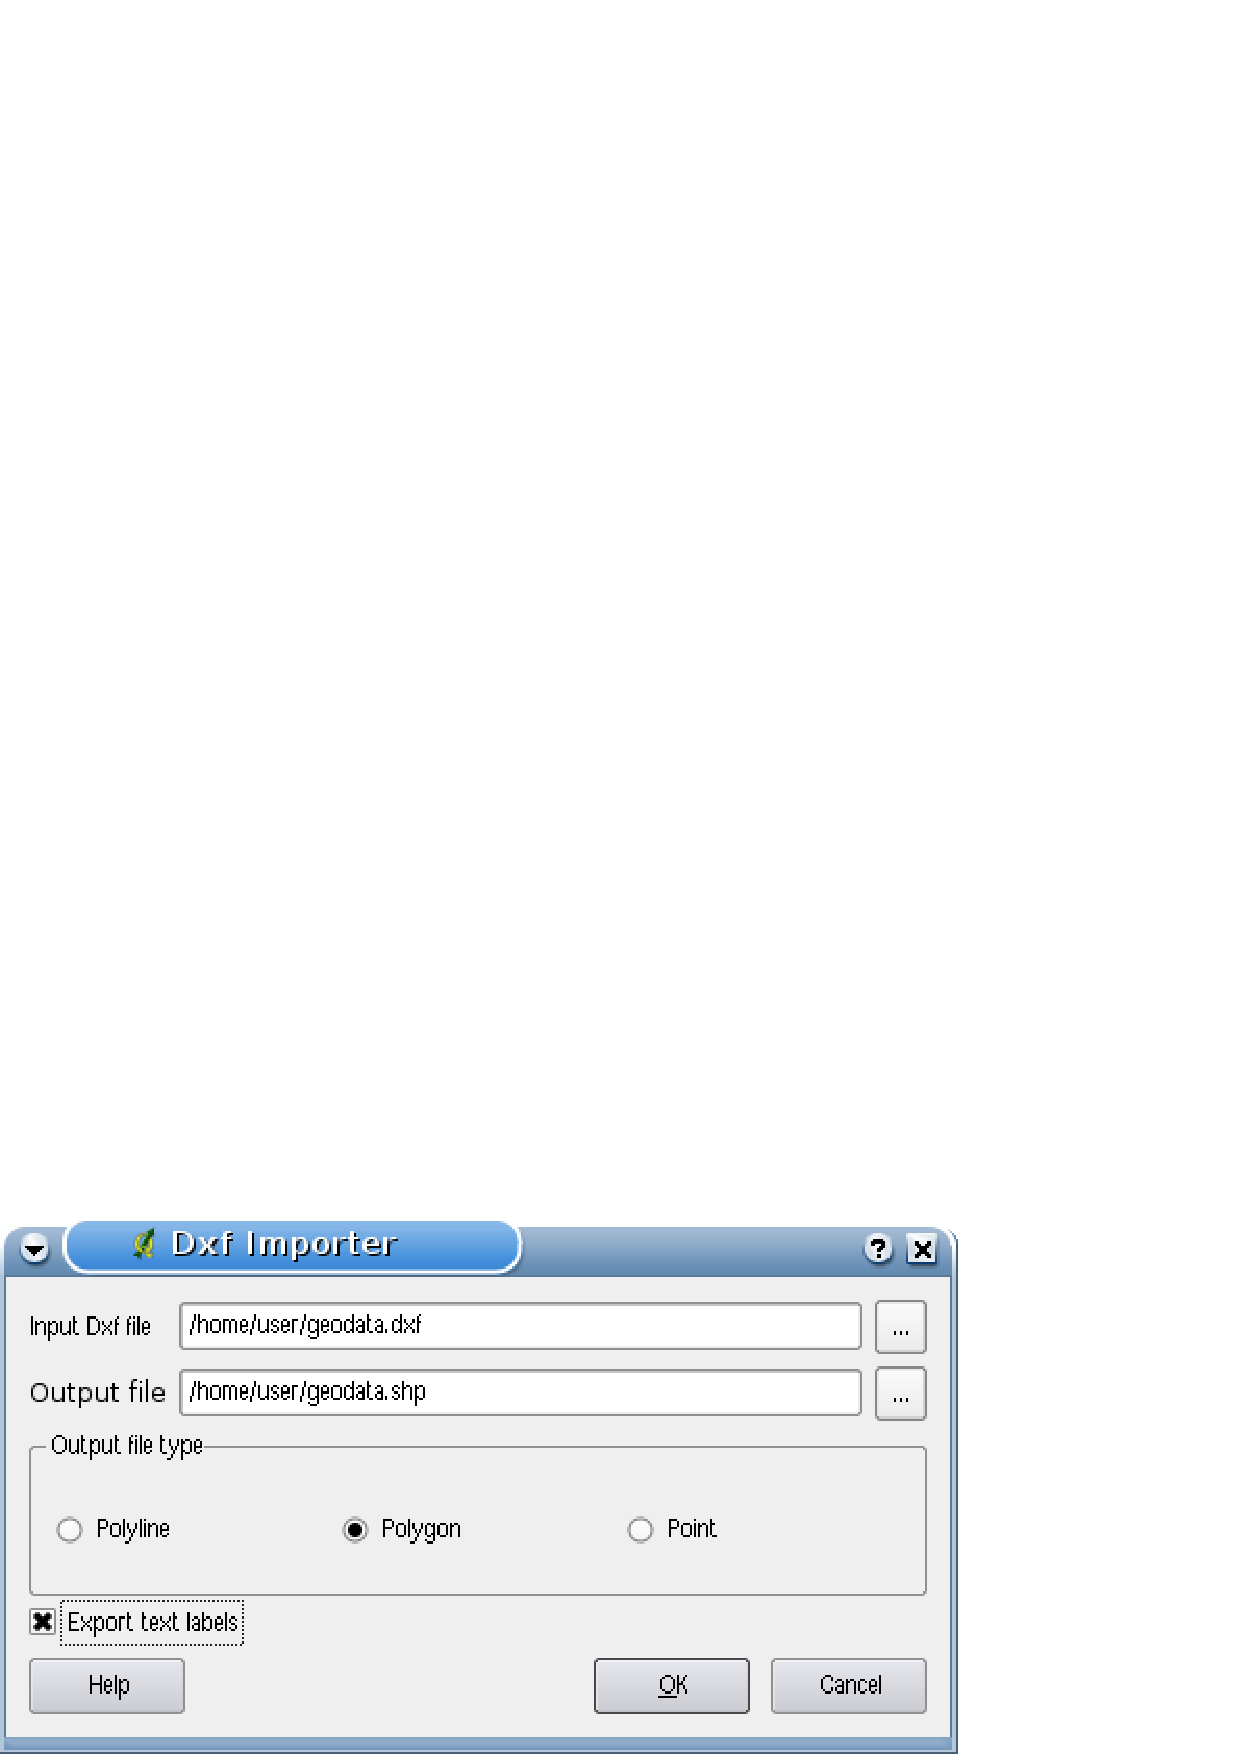
\includegraphics[clip=true, width=12cm]{dxf2shape_dialog}
%\end{center}  
%\end{figure}
\begin{figure}[ht]
   \begin{center}
   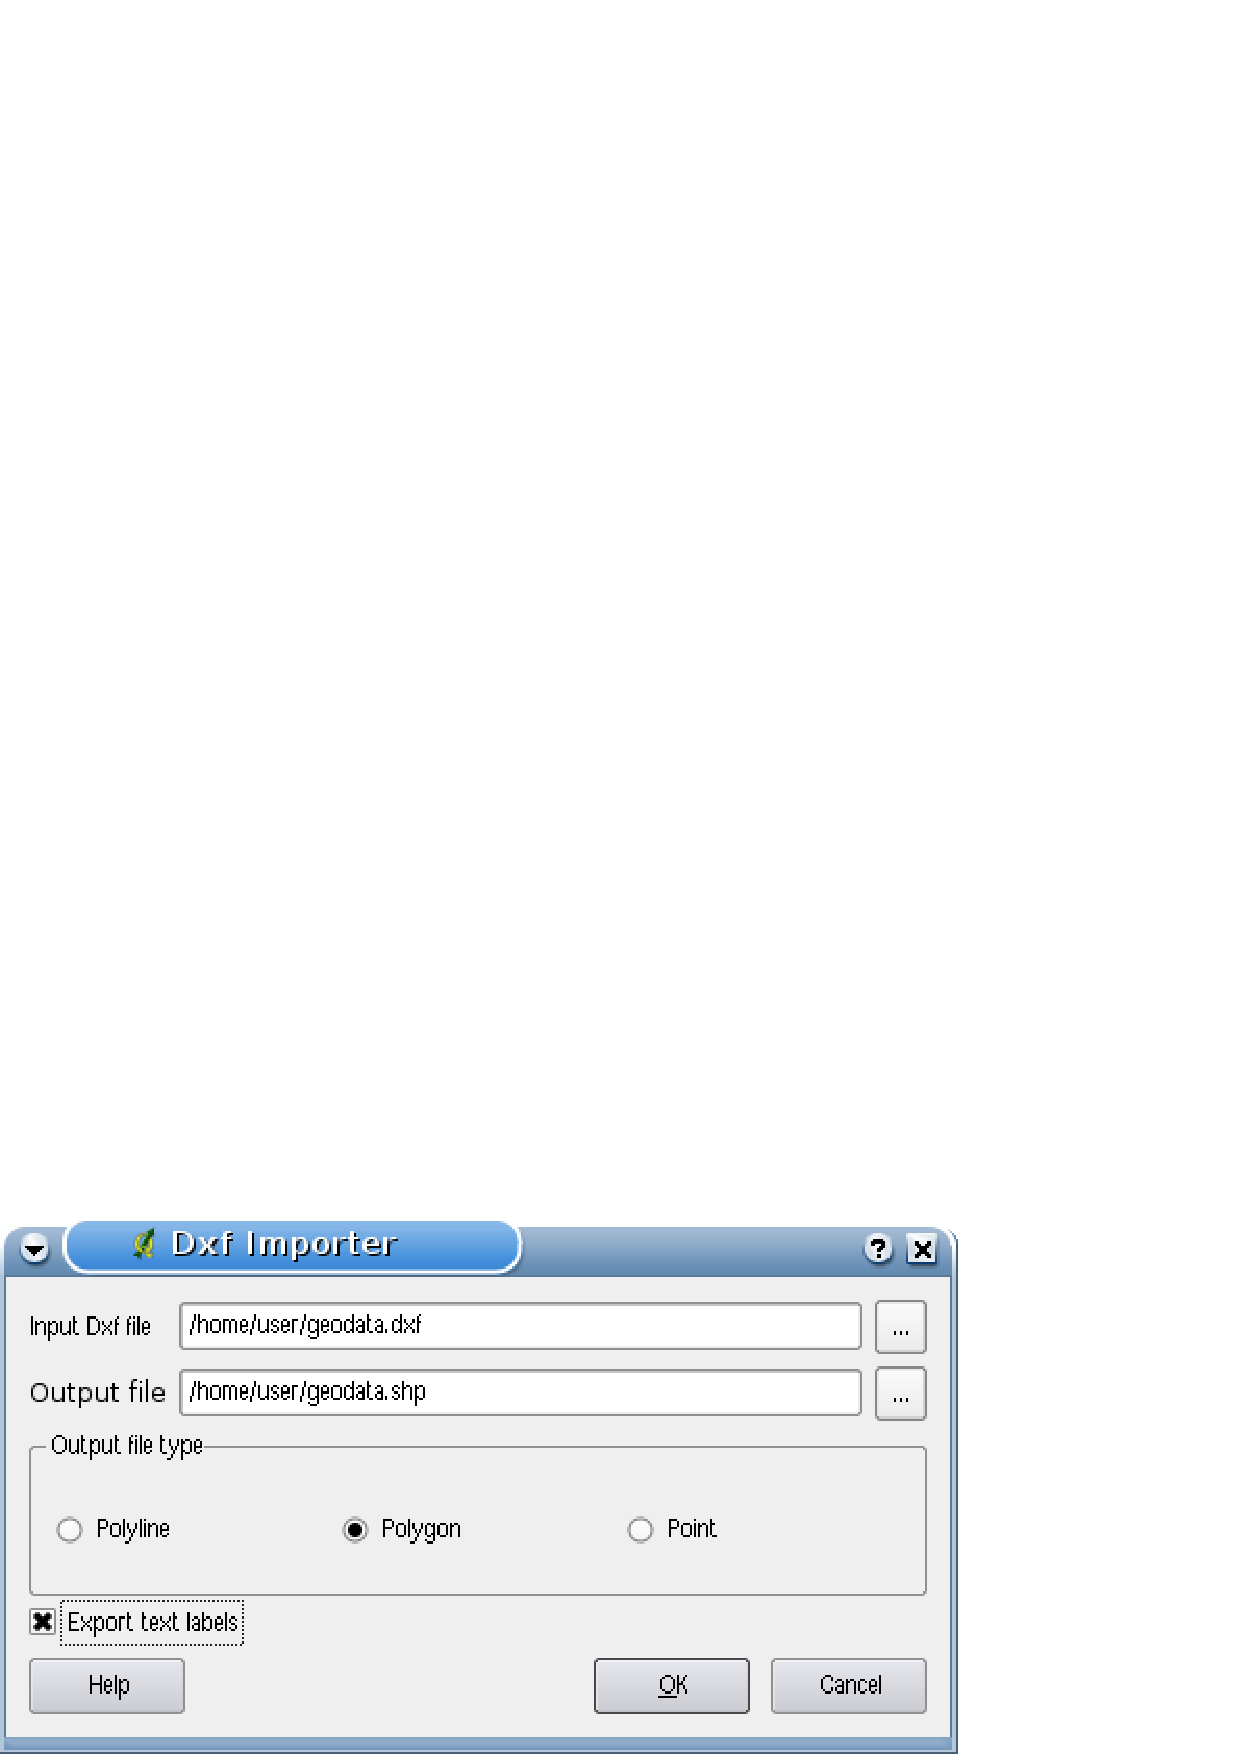
\includegraphics[clip=true, width=12cm]{dxf2shape_dialog}
   \caption{L'extension Convertisseur Dxf2Shape \nixcaption}\label{fig:dxf2shape_dialog}
\end{center}  
\end{figure}

%\minisec{Using the Plugin}
\minisec{Mettre en \oe uvre l'extension}

%\begin{enumerate}
%  \item Start QGIS, load the Dxf2Shape plugin in the Plugin Manager (see Section 
%  \ref{sec:load_core_plugin}) and click on the \toolbtntwo{dxf2shp_converter}{Dxf2Shape Converter} 
%  icon which appears in the QGIS toolbar menu. The Dxf2Shape plugin dialog appears as shown in Figure \ref{fig:dxf2shape_dialog}.
%  \item Enter input DXF file, a name for the output Shapefile and the Shapefile type.
%  \item Enable the \checkbox{Export text labels} checkbox if you want to create an extra point layer with labels.
%  \item Click \button{Ok}. 
%\end{enumerate}
\begin{enumerate}
  \item Démarrez QGIS, chargez l'extension Dxf2Shape dans le gestionnaire 
  d'extensions (voir la Section \ref{sec:load_core_plugin}) puis appuyez sur 
  l'icône \toolbtntwo{dxf2shp_converter}{Convertisseur Dxf2Shape} qui apparaît 
  dans la barre d'outils QGIS. La boîte de dialogue de l'extension Dxf2Shape 
  apparaît alors comme montrée dans la Figure \ref{fig:dxf2shape_dialog}.
  \item Entrez la localisation du fichier DXF ainsi qu'un nom et un type pour 
  le shapefile à créer.
  \item Cochez la case \checkbox{Exporter les étiquettes} si vous souhaitez 
  créer une couche point supplémentaire contenant les étiquettes.
  \item Appuyez sur \button{Ok}. 
\end{enumerate}